\documentclass[10pt,onecolumn]{article}
\usepackage{graphicx}
\usepackage{url}
\usepackage{wrapfig}
\usepackage{tikz}

\title{\vspace{-4.2cm}Software Requirement Specification for Tracking Interconnected Facebook Links }
\author{ ELEN4009 - Software Engineering\\ Julian Zeegers (704582) \\  Joseph Gage (751052)\\ James Allingham (672732) \\ Nathan Haag (873666)}

\addtolength{\oddsidemargin}{-1.5cm}
\addtolength{\evensidemargin}{-.0cm}
\addtolength{\textwidth}{3cm}


%%%%%%%%%%%%%%%%%%%%%%%%%%%%%%%%%%%%%%%%%%%%%%%%%%%%%%%%%%%%%%%%%%%%%%%%%%%%%%%
\begin{document}
\date{\vspace{-5ex}}
\maketitle
\pagestyle{plain}
\setcounter{page}{1}

%%%%%%%%%%%%%%%%%%%%%%%%%%%%%Main Body%%%%%%%%%%%%%%%%%%%%%%%%%%%%%%%%%%%%%%


\section{Introduction}
 

\section{Software Development Life Cycle Choice}



\section{Architecture Choice}


\section{Front-end User Interface Method}


\section{Back-end Service}

The back-end will be based on the \emph{Django} web framework running on an \emph{Apache Web Server}. The DBMS will be \emph{Neo4j}, a graph database, that will be interacted with via the Python driver \emph{Py2neo}. 
\subsection{Django}
\begin{wrapfigure}{r}{0.2\textwidth}
  \begin{center}
    
\includegraphics[width=0.18\textwidth]{django}
  \end{center}
  \caption{The Django Logo}
\end{wrapfigure}


Django is an open source high-level Python Web Framework. It is based on speed, security and scalability. It is also commonly used, with companies such as Mozilla, Pinterest and National Geographic building their websites with it \cite{django}. 

Although it has its own nomenclature, Django can be considered an MVC (Model View Controller) framework and has been compared to the popular \emph{Ruby on Rails} web framework. An MVC framework is based on a three layer abstraction. The first layer abstracts the data access of the web application and is called the Model layer. The second layer is responsible for data display and is called the View layer. The final layer regulates the Views and is called the Controller layer. In Django's nomenclature, the view is equivalent to the standard controller, the template is equivalent to the standard view and the model is much the same as usual. For this reason Django is often referred to as a MTV or Model Template View framework \cite{djangobook}. It is important to note that Django is not a programming language, it is a programming pattern designed to streamline web development in the Python programming language.

Django has its own lightweight web server designed to be used for testing and development. However, for production the Django Software Foundation recommends using Apache with the \emph{mod\_wsgi} module \cite{djangoApache}.
\subsection{Apache}

Apache is a free HTTP web server that has been in production since 1995. It is an extremely sophisticated and flexible tool which supports the newest HTTP standards and a large number of platforms \cite{apache}. Apache has a large number of compiled modules that greatly extend it's functionality. 
\begin{wrapfigure}{r}{0.2\textwidth}
  \begin{center}
    
\includegraphics[width=0.18\textwidth]{apache}
  \end{center}
  \caption{The Apache Logo}
\end{wrapfigure}


Apache processes any incoming HTTP requests from the clients and then sends the appropriate HTTP responses back. This will be done by interfacing with the Django web framework which will make the appropriate decisions based on the requests, and return responses containing content such as information from the Neo4j database. 

Apache has many functions such as virtual hosting which allow one Apache installation to server multiple websites. This feature allows developers of small websites to save on server costs. Apache also provides many useful security features required when a website goes into production such as: password and digital certificate authentication, SSL and TLS support, and many more. For larger websites Apache also allows load balancing. 

\subsection{Neo4j}
Neo4j is a graph database written in Java. It is widely used and has drivers for many languages including Python. Neo4j follows the Atomicity Consistency Isolation Durability (ACID) model which means that it is extremely reliable.  

Graph databases are a type of NoSQL or Not Only SQL database. They excel at managing large complex sets of data which can be described as nodes and relationships. Figure \ref{neo4eg} shows an example of the type of data that can be stored in a graph database.

\begin{figure}[htbp]
    \centering
    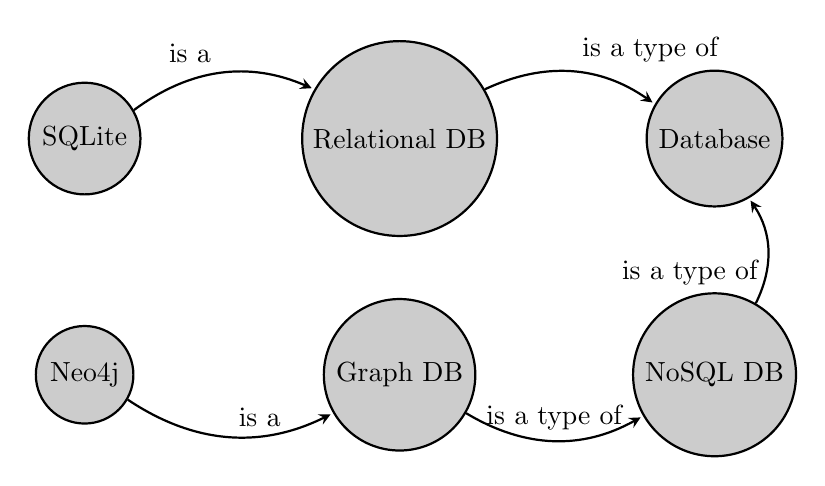
\begin{tikzpicture}[->,>=stealth,shorten >=1pt,auto,node distance=3cm,
       thick,main node/.style={circle,fill=black!20,draw}]

      \node[main node] at (0,0) (1) {Neo4j};
      \node[main node] at (4,0) (2)  {Graph DB};
      \node[main node] at (8,0) (3) {NoSQL DB};
      \node[main node] at (8,3) (4) {Database};
      \node[main node] at (4,3) (5) {Relational DB};
      \node[main node] at (0,3) (6) {SQLite};
      \path
      (1) edge [bend right] node {is a} (2)
      (2) edge [bend right] node {is a type of} (3)
      (3) edge [bend right] node {is a type of} (4)
      ;
      \path 
      (6) edge [bend left] node {is a} (5)
      (5) edge [bend left] node {is a type of} (4)
      ;

    \end{tikzpicture}
    \caption{Example of data stored in a graph database}
    \label{neo4eg}
\end{figure}

In this application the data being stored will be that of Facebook relationships. Graph databases are orders of magnitudes faster than a RDBMS for queries on this kind of data, such as finding extended friend networks of individuals \cite{graphdbs}.  Figure \ref{friends} shows an example of the kind of data that will be stored in the database.

\begin{figure}[htbp]
    \centering
    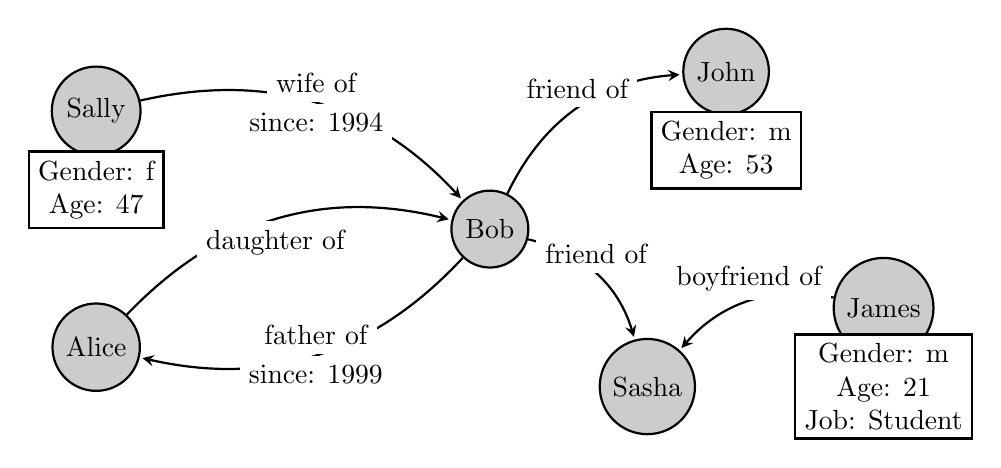
\begin{tikzpicture}[->,>=stealth,shorten >=1pt,auto,thick,main node/.style={circle,fill=black!20,draw,align=center}]

      \node[main node] at (-1,-0.5) (1) {Sally};
      \node[draw,rectangle, below of = 1, align=center,fill=white] (7) {Gender: f\\ Age: 47};
      \node[main node] at (7,0) (2)  {John};
      \node[draw,rectangle, below of = 2, align=center, fill=white] (6) {Gender: m\\ Age: 53};
      \node[main node] at (4,-2) (3) {Bob};
      \node[main node] at (-1,-3.5) (4) {Alice};
      \node[main node] at (6,-4) (5) {Sasha};
      \node[main node] at (9,-3) (8) {James};
      \node[draw,rectangle, below of = 8, align=center, fill=white] (9) {Gender: m\\ Age: 21\\ Job: Student};

    
      \path
      (1) edge[bend left] node[above, fill=white] {wife of} node[below,fill=white] {since: 1994} (3)
      (3) edge[bend left] node[above,fill=white] {friend of} (5)
      (3) edge[bend left] node[above,fill=white] {father of} node[below,fill=white] {since: 1999} (4)
      (3) edge[bend left] node[above,fill=white] {friend of} (2)
      (8) edge[bend right] node[above,fill=white] {boyfriend of} (5)
      (4) edge[bend left] node[below,fill=white] {daughter of} (3)
      ;

    \end{tikzpicture}
    \caption{Example of facebook type data in a graph database}
    \label{friends}
\end{figure}
From Figure \ref{friends} notice that both the relationships as well as the entities themselves have associated data. In face each entity acts as a key value store. Queries can be performed to find all friends since a certain date or all friends of friends (as discussed above). These queries can be performed using Neo4j's \emph{Cypher} query language or via language drivers. The language driver that will be used for this application is \emph{Py2neo}.

\section{Supporting Software}


\begin{thebibliography}{1}
\bibitem{django} Django Software Foundation. "Django Overview". \url{https://www.djangoproject.com/start/overview/}. 2016. Last accessed: 9 March 2016. 
\bibitem{djangobook} Adrian Holovaty, Jacob Kaplan-Moss, et al. "The Django Book". \url{http://www.djangobook.com/en/2.0/index.html#}. Ch 3. Last accessed: 9 March 2016.
\bibitem{djangoApache} Django Software Foundation. "How to install Django". \url{https://docs.djangoproject.com/en/1.9/topics/install/}. 2016. Last accessed: 9 March 2016.	
\bibitem{apache} Apache Software Foundation. "Apache - HTTP Server Project". \url{https://httpd.apache.org/ABOUT_APACHE.html}. 2016. Last accessed: 9 March 2016.	
\bibitem{graphdbs} Robinson I, Webber J, Eifrem E. "Graph Databases" O'Reilly Media. ch 2. pp 21 - 22. June 2013.`:w
 
\end{thebibliography}

 %%%%%%%%%%%%%%%%%%%%%%%%%%%%%%%%%%%%%%%%%%%%%%%%%%%%%%%%%%%%%%%%%%%%%%%%%%%%%%
\clearpage
\end{document}
